%CHAPTER
\chapter{Implementace úložiště}
Výsledné řešení by mělo obsahovat dvě databáze, pomocí kterých bude možno vyhledávat patenty, ať už podle určitých atributů (ID, země, obor, a jiné), nebo pomocí full-textu. Vybrané databáze jsou uzpůsobeny pro ukládání velkého množství patentových dat, které byly staženy z národních zdrojů. 
\newline
\indent Import dat bude řešen pomocí vlastní aplikace, která bude filtrovat nevalidní patenty (neexistující povinné atributy, nevalidní \gls{XML} struktura, ...) a importovat validní patenty do databází. Pro MySQL databázi bude potřeba z patentu získat pouze specifické atributy.
\newline
\indent Výsledné řešení bude potřeba jednoduše nasadit na produkční server / počítač, aniž by bylo potřeba instalovat vícero aplikací. Řešení se postará o automatickou instalaci obou databází, jejich inicializaci (vytvoření tabulek, kolekcí, pohledů, ...) a zajistí propojení mezi databází \textbf{MongoDB} a full-textovým vyhledávačem \textbf{Elasticsearch}. S databázemi se zároveň nainstalují i aplikace pro jejich správu.

\section{Implementace databáze}
Pro databázi \textbf{MySQL} bylo navrženo a vytvořeno databázové schéma tak, aby bylo možno použít co nejvíce atributů při filtrování patentů pro statistiky. V \textbf{MongoDB} bude vytvořena databáze s jednou kolekcí, která bude obsahovat všechny vyfiltrované patenty.
\subsection{MongoDB}
Pro MongoDB byla použita jedna z nejnovějších verzí komunitní edice (verze 5.0.6). Programový systém \textbf{Mongo-express} (verze 0.54.0) bude použit jako nástroj pro spravování MongoDB databáze, ke kterému lze přistoupit pomocí webového prohlížeče.
\newline
\indent V databázovém schématu byla vytvořena databáze s názvem \textbf{patents}, která obsahuje pouze jednu kolekci s názvem \textbf{patents}. V této kolekci budou uloženy všechny vyfiltrované patenty ze všech zemí. Vzhledem k tomu, že MongoDB bude sloužit jen jako uložiště patentových dat, tak není potřeba vytvářet více kolekcí nebo databází. Jako další důvod pro zvolení pouze jedné kolekce je počet indexů v Elasticsearch, kdy byl použit pouze jeden index pro zaindexování všech dat. Důvod je takový, že chceme vždy prohledávat všechny patenty a ne jen jejich část, takže vícero indexů by akorát způsobovalo pomalejší zpracování dotazů pro vyhledávání.

\subsection{MySQL} \label{subsec:mysql_impl}
Pro MySQL byla použita verze komunitního serveru (verze 8.0.16). Programový systém \textbf{phpMyAdmin} (verze 5.1.3)  bude použit jako nástroj pro spravování MySQL databáze, ke kterému lze přistoupit pomocí webového prohlížeče. Lze použít i nástroj \textbf{MySQL Workbench} pro správu MySQL databáze, ale pro naše účely bohatě postačí \textbf{phpMyAdmin}.
\newline
\indent Schéma splňuje pouze druhou normální formu. Je to z toho důvodu, že tabulka \textbf{classification} obsahuje některé duplicitní hodnoty ve sloupcích. Duplicitu samozřejmě lze odstranit, ale zvýšilo by to složitost celého systému - \gls{SQL} dotazy by byly složitější a pomalejší v případě příkazu \textit{SELECT}, který by vyhledával data z několika tabulek, spojených příkazem \textit{JOIN}.
\newline

\noindent Databázové schéma pro MySQL lze vidět na obrázku č. \ref{fig:mysql_schema}.
\begin{figure}[H]
\centering
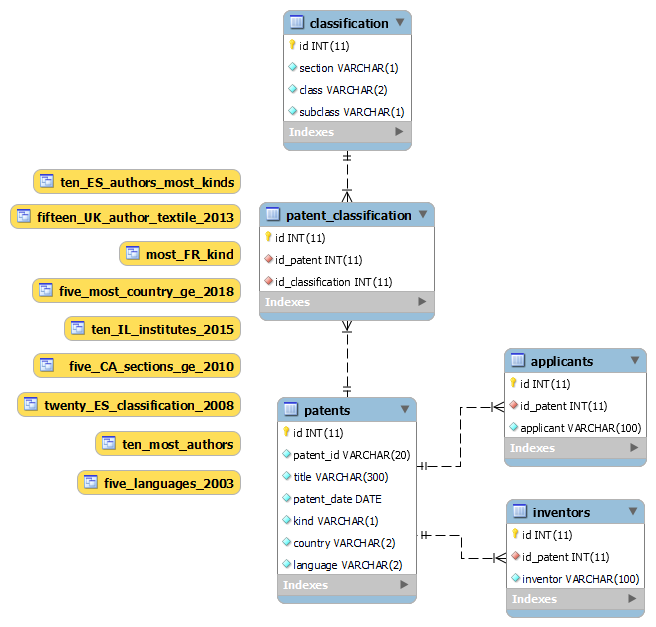
\includegraphics[width=12cm]{img/eer}
\caption{Schéma pro MySQL databázi.}
\label{fig:mysql_schema}
\end{figure}

\subsubsection{Tabulka patents}
Tabulka \textbf{patents} uchovává všechny národní patenty, které byly poskytnuty zdarma a obsahují všechny povinné atributy.

\subsubsection{Tabulka classification}
Tabulka \textbf{classification} slouží k uchovávání \gls{IPC} klasifikace daného patentu, konkrétně jeho sekci, třídu a podtřídu (skupina a podskupina vybrána nebyla, protože se vyskytovala v patentech jen ojediněle). 

\subsubsection{Tabulka patent\_classification}
Tabulka \textbf{patent\_classification} má kardinalitu \textit{M:N} a slouží jako propojení tabulky \textbf{patents} a tabulky \textbf{classification}. Jeden patent může mít více klasifikací (například se mohlo změnit označení v průběhu let, nebo patent pokrývá více oborů) a jedna klasifikace může být u více patentů.

\subsubsection{Tabulka inventors}
Tabulka \textbf{inventors} slouží k uchovávání jmen autorů patentů. Kardinalita mezi tabulkou \textbf{patents} a tabulkou \textbf{inventors} je \textit{1:N}, protože pro jeden patent může existovat více autorů.

\subsubsection{Tabulka applicants}
Tabulka \textbf{applicants} slouží k uchovávání jmen žadatelů patentů. Ačkoli existuje tabulka pro autory, tak může existovat scénář, ve kterém bude potřeba vyhledávat žadatele pro daný patent. Kardinalita mezi tabulkou \textbf{patents} a tabulkou \textbf{applicants} je \textit{1:N}, protože pro jeden patent může existovat více žadatelů.

\subsubsection{Pohledy}
Pohled je databázový objekt, který uživateli poskytuje data ve stejné podobě jako tabulka. Stručněji řečeno, je to struktura uchovávající \gls{SQL} dotaz, který se většinou dotazuje dané tabulky na specifická data.
\newline
\indent V databázi pro patenty bylo vytvořeno celkem devět pohledů, kdy každý z nich reprezentuje jeden scénář, který je použit při ověřování efektivního vytěžování (viz kapitola č. \ref{sec:efektivni_vytezovani_sql}).

\section{Nasazení úložiště}
Celý modul našeho úložiště čítá celkem 5 nástrojů - MySQL, MongoDB, Elasticsearch, phpMyAdmin a Mongo-express. Zároveň bude potřeba nastavit připojení mezi MongoDB a Elasticsearch tak, aby při přidání nového patentu do databáze byl následně zaindexován ve full-textovém vyhledávači. Pokud bychom měli po každém uživateli chtít instalaci všech těchto nástrojů a k tomu stahovat další nástroje pro vytvoření připojení mezi MongoDB a Elasticsearch, tak to zabere mnoho času a existuje zde velká pravděpodobnost že některé nástroje nebudou kompatibilní s aktuální verzí operačního systému. Z těchto důvodů byl zvolen software \textbf{Docker}, pomocí kterého se provede veškerá instalace a nastavení automaticky.

\subsection{Docker}
\textbf{Docker} je jeden z nejznámějších open-source nástrojů pro dodání aplikací v balíčkách zvaných \textit{kontejner}. \textbf{Docker} využívá virtualizaci na úrovni operačního systému, čímž je výrazně snížena režie na rozdíl od klasických virtuálních strojů. Existují i jiné alternativy než docker, ale díky velké popularitě a fanouškovské základně byl vybrán právě docker.
\newline
\indent Definice a instalace aplikací je zajištěna pomocí nástroje \textbf{Docker compose}. Definice probíhá pomocí souboru s názvem \textit{docker-compose.yml} (viz obrázek č. \ref{fig:compose}), který využívá \gls{YAML} formát pro serializaci strukturovaných dat. V docker-compose.aml souboru pro tento modul je definováno celkem devět aplikací a dva nastavovací moduly. Data nejsou součástí inicializace kontejnerů, je potřeba je importovat dodatečně (dále viz kapitola \textbf{Uživatelská dokumentace}).
\begin{figure}[H]
\centering
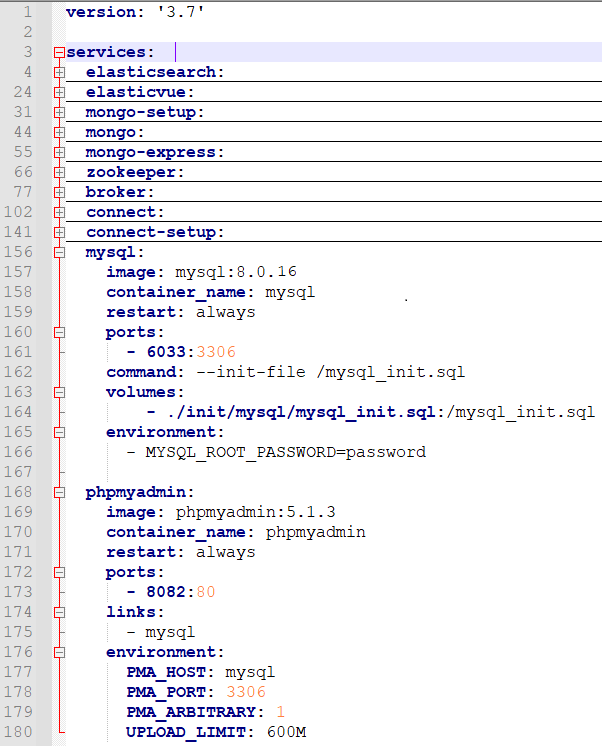
\includegraphics[width=11cm]{img/compose}
\caption{Ukázka souboru docker-compose.yml.}
\label{fig:compose}
\end{figure}

\subsubsection{Docker - Elasticsearch}
Pro Elasticsearch byly nadefinovány dvě aplikace:
\begin{itemize}
\item \textbf{elasticsearch} - Oficiální image full-textového vyhledávače Elasticsearch ve verzi 8.2.0. V nastavení byla vypnuto zabezpečení kvůli problémům se sadou replik v MongoDB.
\item \textbf{elasticvue} - Grafické uživatelské rozhraní pro Elasticsearch ve verzi 0.39.0, dostupné na localhostu na portu 8080.
\end{itemize}

\subsubsection{Docker - MongoDB}
Pro MongoDB byly nadefinovány dvě aplikace a jeden nastavovací modul:
\begin{itemize}
\item \textbf{mongo} - Oficiální image databáze MongoDB ve verzi 5.0.6. V databázi bylo nutné nastavit sadu replik, aby bylo možné vytvořit propojení mezi MongoDB a Elasticsearch.
\item \textbf{mongo-express} - Grafické uživatelské rozhraní pro MongoDB ve verzi 0.54.0, dostupné na localhostu na portu 8081.
\item \textbf{mongo-setup} - Nastavovací modul pro MongoDB, který po inicializaci databáze inicializuje sadu replik a následně vytvoří novou databázi a kolekci pro patenty.
\end{itemize}

\subsubsection{Docker - MongoDB a Elasticsearch konektor}
Pro konektor mezi MongoDB a Elasticsearch byly nadefinovány tři aplikace a jeden nastavovací modul:
\begin{itemize}
\item \textbf{broker} - Komunitní verze Apache Kafka od firmy Confluent ve verzi 6.1.0.
\item \textbf{zookeeper} - Nástroj pro Apache Kafka ve verzi 6.1.0, který funguje jako centralizovaná služba a slouží k údržbě jmenných a konfiguračních dat. Zároveň zajišťuje i flexibilní a robustní synchronizaci v rámci distribuovaných systémů.
\item \textbf{connect} - Nástroj pro Apache Kafka ve verzi 6.1.0, který má za úkol propojit externí systémy s Apache Kafka za pomoci konektorů.
\item \textbf{connect-setup} - Nastavovací modul pro Kafka connect, který po inicializaci Kafka connect vytvoří dva konektory:
	\begin{itemize}
	\item \textit{mongo-source-connector} - Konektor, který aktivně získává nová data z MongoDB a vkládá je do Kafka brokera.
	\item \textit{elasticsearch-sink-connector} - Konektor, který aktivně získává nová data z Kafka brokera a vkládá je do Elasticsearch.
	\end{itemize} 
\end{itemize}

\subsubsection{Docker - MySQL}
Pro MySQL byly nadefinovány dvě aplikace:
\begin{itemize}
\item \textbf{mysql} - Oficiální image databáze MySQL ve verzi 8.0.16. Při inicializaci databáze se vytvoří všechny tabulky i pohledy.
\item \textbf{phpmyadmin} - Grafické uživatelské rozhraní pro MySQL ve verzi 5.1.3, dostupné na localhostu na portu 8082. V nastavení byl navýšen limit pro import souborů na 600 MB z původních 2 MB.
\end{itemize}

\subsection{Inicializace MySQL}
Inicializace MySQL probíhá po vytvoření databáze v rámci docker kontejneru pro MySQL. Pro inicializaci byl vytvořen soubor \textbf{mysql\_init.sql}, který obsahuje příkazy pro vytvoření všech pěti tabulek (názvy tabulek, názvy sloupců, jejich omezení a klíče) a všech devíti pohledů.

\subsection{Inicializace MongoDB}
Inicializace MongoDB probíhá po vytvoření databáze v rámci docker kontejneru \textbf{mongo-setup}, protože MongoDB nemá žádnou možnost jak vložit inicializační soubor při startu kontejneru. Pro inicializaci byly vytvořeny dva soubory:
\begin{itemize}
\item \textbf{create\_mongo\_database.js} - Javascriptový soubor, který obsahuje příkazy pro vytvoření kolekce v databázi pro patenty.
\item \textbf{mongo\_init.sh} - Shell skript, který inicializuje sadu replik v databázi a následně spustí javascriptový soubor \textbf{create\_mongo\_database.js}.
\end{itemize}

\subsection{Propojení MongoDB a Elasticsearch}
Pro propojení MongoDB a Elasticsearch byly vyzkoušeny dva nástroje: \textbf{Mongo-connector} a \textbf{Apache Kafka}. 

\subsubsection{Mongo-connector}
Mongo-connector je obecný připojovací systém vyvinutý firmou MongoDB Inc. v roce 2012, který slouží pro integraci databáze MongoDB s jiným systémem, který podporuje \gls{CRUD} operace. Mongo-connector byl následně udržován pouze komunitně přibližně do roku 2018, kdy byla vydána poslední verze tohoto nástroje (verze 3.1.1).
\newline
\indent V původní verzi úložiště byl mongo-connector použit k propojení MongoDB ve verzi 5.0.6 a Elasticsearch ve verzi 7.17.0. Konektor pracoval rychle a bez problémů do té doby, než bylo potřeba použít novější verzi Elasticsearch (verze 8.x.x), kdy konektor nedokázal navázat žádné spojení a tím pádem nebylo možné využívat vyhledávač.
\newline
\indent Přechod na novější verzi Elasticsearch bylo potřeba z důvodu různých struktur patentů. Národní patentové úřady poskytují svá patentová data v různých strukturách, které se mohou měnit v průběhu let, což byl i jeden z důvodů pro výběr databáze MongoDB. V případě Elasticsearch je ale nutné, aby data měla stále stejnou strukturu, alespoň v rámci MongoDB kolekcí, protože Elasticsearch si data z kolekcí musí nejdříve zaindexovat pomocí mapperu a pak až v nich lze vyhledávat. V nejnovější verzi Elasticsearche (verze 8.x.x) je použit jiný způsob indexování souborů, takže data mohou mít libovolné struktury. Z tohoto důvodu byl mongo-connector zamítnut a musel být použit nový nástroj Apache Kafka.

\subsubsection{Apache Kafka}
Apache Kafka je distribuované úložiště událostí a platforma pro zpracování datových proudů (streamů). V diplomové práci byla použita Apache Kafka od firmy Confluent, která obsahuje dodatečné komunitní a komerční funkce navržené tak, aby vylepšily streamování operátorů i vývojářů v produkčním prostředí.
\newline
\indent Inicializace konektorů pro Apache Kafka probíhá v nastavovacím modulu \textbf{connect-setup}, ve kterém je stažen a nainstalován program \textbf{CURL}, který je využit shellovým skriptem \textbf{connect.sh}. Tento skript posílá dvě \gls{HTTP} POST metody na brokera (Apache Kafka), pomocí kterých se vytváří nové konektory. Na obrázku č. \ref{fig:sink} lze vidět data ve formátu JSON pro POST metodu, která vytvoří spojení z Apache Kafka do Elasticsearch, a na obrázku č. \ref{fig:source} lze vidět data pro vytvoření spojení z MongoDB do Apache Kafka.
\begin{figure}[H]
\centering
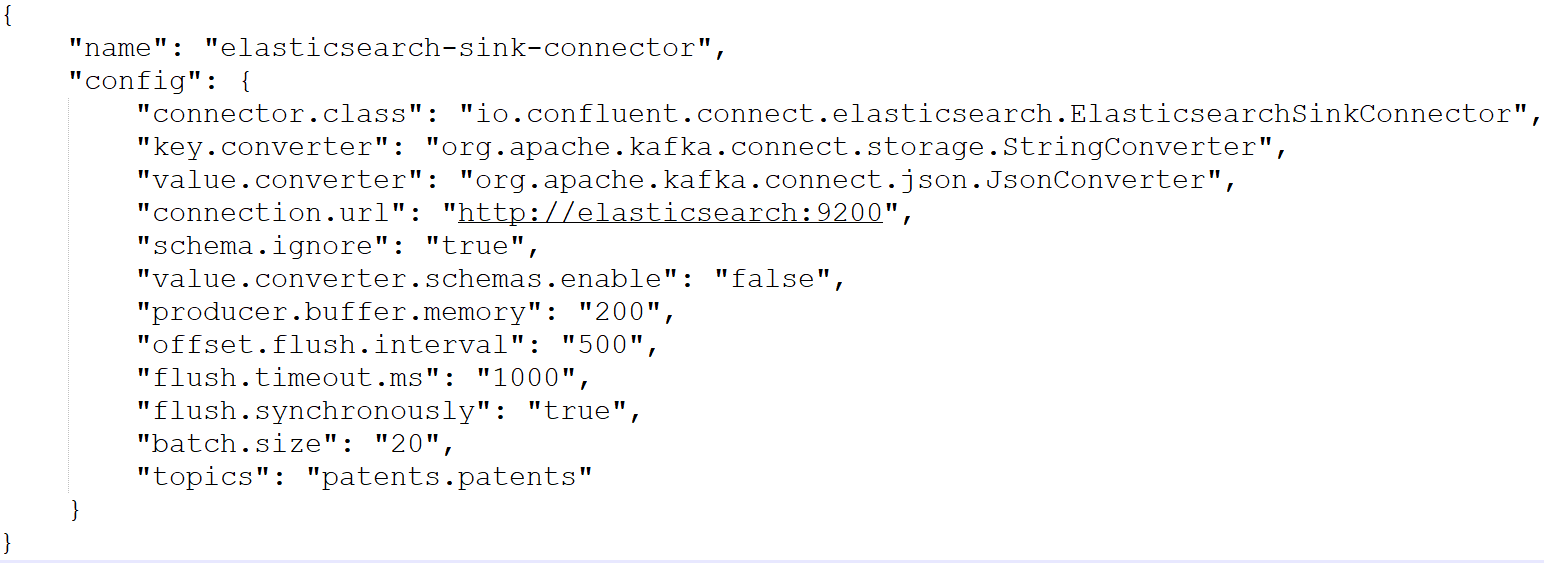
\includegraphics[width=12cm]{img/sink}
\caption{Data pro vytvoření konektoru z Apache Kafka do Elasticsearch.}
\label{fig:sink}
\end{figure}
\begin{figure}[H]
\centering
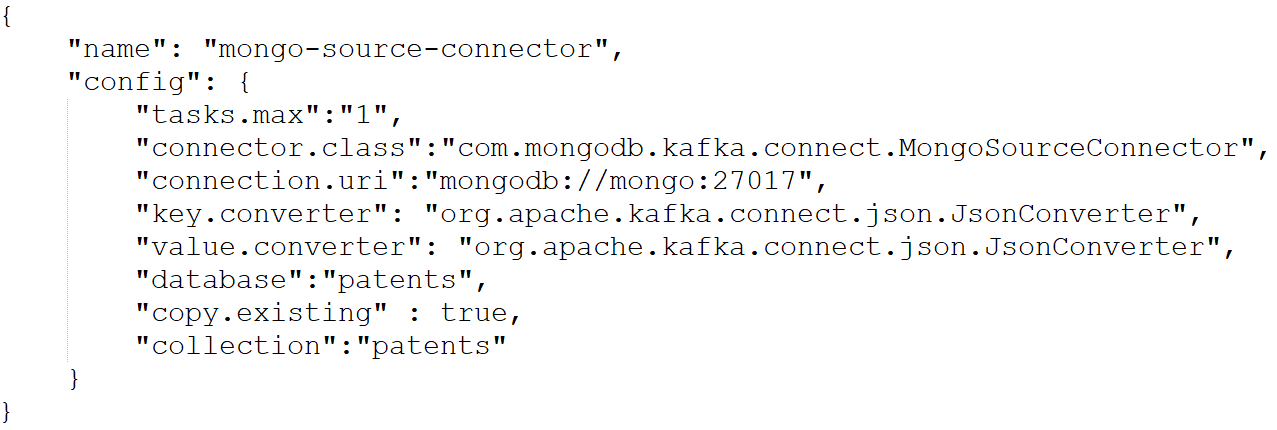
\includegraphics[width=11cm]{img/source}
\caption{Data pro vytvoření konektoru z MongoDB do Apache Kafka.}
\label{fig:source}
\end{figure}